\section{Flussnetzwerke und Maximum-Flow}

\begin{wrapfigure}{r}{0.2\textwidth}
	\centering
	\vspace{-20pt}
	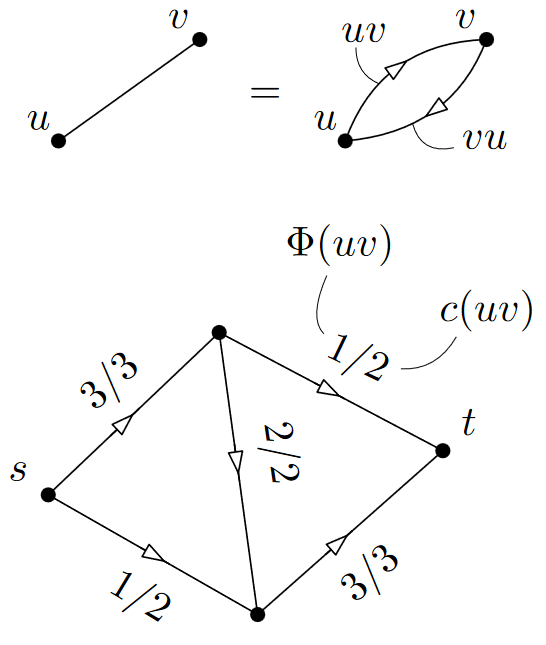
\includegraphics[width=0.2\textwidth]{images/fnet.png}
	\vspace{40pt}
	\vspace{-800pt}
\end{wrapfigure}

Wir betrachten im Folgenden gerichtete Graphen $D=(V,A)$
\begin{itemize}
	\item Kante von $u$ nach $v$ heißt $uv$ und es gilt $uv\neq vu$
	\item Wir nehmen an, dass $uv\in A\iff vu\in A$
\end{itemize}
\bigskip
\textbf{Definition}: Ein \textbf{Flussnetzwerk} ist ein 4-Tupel $$(D=(V, A), c\colon A\rightarrow \R_{>0}, s\in V, t\in V )$$ wobei $D$ wie oben, $c$ jeder Kante ihre Kapazität zuordnet, $s$ die Quelle und $t$ die Senke darstellen. Die Kapazität einer Kante ist in beide Richtungen gleich, also $$c(uv)=c(vu)\quad \forall uv\in A$$

\textbf{Definition}: Ein \textbf{$\boldsymbol{s}$-$\boldsymbol{t}$-Fluss} bezüglich eines Flussnetzwerkes ist eine Funktion $\Phi\colon A\rightarrow\R$, die jeder Kante $uv$ ihren Fluss von $u$ nach $v$ zuordnet und Folgendes einhält: 
\begin{itemize}
	\item \underline{Flusserhaltung}: $\sum\limits_{uv\in A}\Phi(uv)=0$ für jeden Knoten $u\neq s,t$
	
	(Netto-Ausfluss aus $u$ muss 0 sein, da Einfluss negativ gezählt wird)
	\item \underline{Zulässigkeit}: $\Phi(uv)\leq c(uv)$ für alle $uv\in A$
	\item \underline{Antisymmetrie}: $\Phi(uv)=-\Phi(vu)$ für alle $uv\in A$
\end{itemize}
Der \textbf{Wert} von $\Phi$ ist der Netto-Ausfluss bei $s$: $\Phi(s)=\sum\limits_{sv\in A}\Phi(sv)=-\Phi(t)$

\texttt{MAXIMUM-FLOW}: Gegeben ein Flussnetzwerk, finde einen maximalen s-t-Fluss. Im Allgemeinen in $\mathcal{O}(n^2)$, aber für planare Graphen geht es besser.\\

\textbf{Notation}: Für $X\subseteq V$ sei $\Phi(X)\coloneqq \sum\limits_{\substack{uv\in A \\ u\in X, v\notin X}}\Phi(uv)$ der Netto-Ausfluss aus $X$. 

Also ist $\Phi(\{s\})=\Phi(s)$ und $\Phi(\{v\})=0$ für alle $v\neq s,t$.\\

\textbf{Beobachtung}: Sind $X,Y\subseteq V$ disjunkt, so gilt $\Phi(X\cup Y)=\Phi(X)+\Phi(Y)$ Zerlegt man $X$ in einelementige Mengen, so folgt $\Phi(X)=\sum\limits_{u\in X}\Phi(u)$.
\begin{center}
	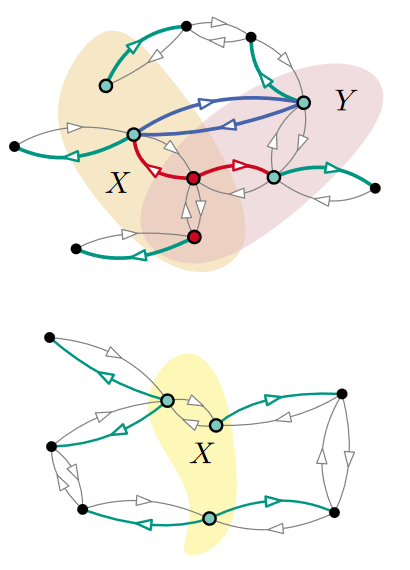
\includegraphics[width=0.2\textwidth]{images/fnet-2.png}
\end{center}

\begin{wrapfigure}{r}{0.2\textwidth}
	\centering
	\vspace{0pt}
	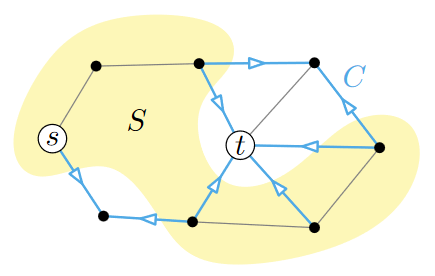
\includegraphics[width=0.2\textwidth]{images/s-t-cut.png}
	\vspace{40pt}
	\vspace{-800pt}
\end{wrapfigure}
\textbf{Definition}: Ein \textbf{$\boldsymbol{s}$-$\boldsymbol{t}$-Schnitt} ist ein Schnitt $C\subseteq A$, induziert von einer Knotenmenge $S\subseteq V$ mit $s\in S,t\notin S$:
$$C\coloneqq\{uv\in A\mid u\in S, v\notin S\}$$
Die \textbf{Kapazität} eines solchen Schnitts ist $c(C)\coloneqq \sum\limits_{e\in C}c(e)$.\\


\textbf{Max-Flow-Min-Cut-Lemma}: Für jeden $s$-$t$-Schnitt $C$ und $s$-$t$-Fluss $\Phi$ gilt $$\Phi(s)\leq c(C)$$

\textit{Beweis}: $\Phi(s)=\sum\limits_{v\in S}\Phi(\{v\})=\Phi(S)=\sum\limits_{e\in C}\Phi(e)\leq\sum\limits_{e\in C}c(e)=c(C)$

wobei die erste Gleichheit gilt, da $\Phi(\{v\})=0$ für alle $v\neq s$ ist.\\

\textbf{Max-Flow-Min-Cut-Theorem}: $\max\Phi(s)=\min c(C)\qquad$ \textit{ohne Beweis.}\\
\begin{wrapfigure}{r}{0.2\textwidth}
	\centering
	\vspace{-20pt}
	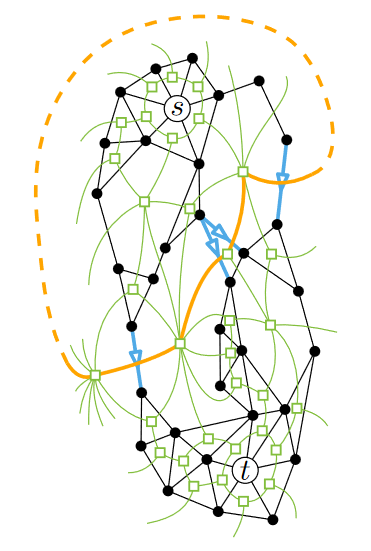
\includegraphics[width=0.25\textwidth]{images/cut-circ.png}
	\vspace{40pt}
	\vspace{-80pt}
\end{wrapfigure}
Im Folgenden reicht es also nach einen $s$-$t$-Schnitt mit minimaler Kapazität zu suchen. Da $c(e)>0$ für jede Kante $e\in A$, reicht es inklusionsminimale $s$-$t$-Schnitte $C\subseteq A$ zu betrachten, also solche, die keinen $s$-$t$-Schnitt enthalten. Schnitte in $D$ entsprechen Kreise im Dualgraphen.\\

\textbf{Definition}: Der \textbf{gerichtete Dualgraph} $D^*=(V^*,A^*)$ zu $D$: Für $e=uv$ in $D$ sei links($e$) und rechts($e$) die links bzw. rechts von $e$ liegende Facette, wenn man über $e$ von $u$ nach $v$ geht. In $D^*$ sei die Dualkante $e^*$ von links($e$) nach rechts($e$) orientiert.
\begin{center}
	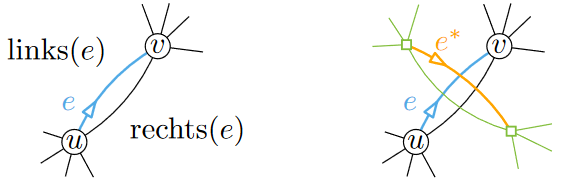
\includegraphics[width=0.4\textwidth]{images/dir-dual.png}
\end{center}
\bigskip
\textbf{Definition}: Ein \textbf{$\boldsymbol{s}$-$\boldsymbol{t}$-Kreis} ist ein einfacher gerichteter Kreis in $D^*$ mit $s$ auf der rechten und $t$ auf der linken Seite.

\begin{wrapfigure}{r}{0.15\textwidth}
	\centering
	\vspace{-35pt}
	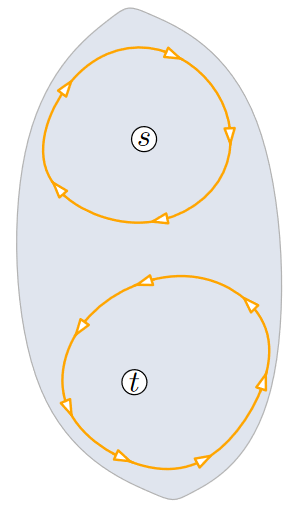
\includegraphics[width=0.15\textwidth]{images/s-t-circ.png}
	\vspace{30pt}
	\vspace{-80pt}
\end{wrapfigure}

\textbf{Lemma}: Sei $C\subseteq A$ eine Kantenmenge und $C^*\subseteq A^*$ die dazu duale Kantenmenge. Dann gilt:
$$C \text{ ist ein }s\text{-}t\text{-Schnitt}\iff C^* \text{ ist ein }s\text{-}t\text{-Kreis}$$
Wir setzen $l(e^*)\coloneqq c(e)$ für alle $e\in A$ und interpretieren das als Länge der Dualkante $e^*$.

Es reicht also einen $s$-$t$-Kreis mit minimaler Länge zu finden. 

\textbf{Satz}: Für planare Graphen mit $s$ und $t$ an einer gemeinsamen Facette, kann ein Max-Flow in Linearzeit gefunden werden.

\textit{Beweis}:
\begin{itemize}
	\item O.B.d.A. liegen $s$ und $t$ an der äußeren Facette
	\item Jeder $s$-$t$-Kreis muss die äußere Facette $f_0$ als Dualknoten enthalten
	\item Füge neue Kante $e_0=st$ mit Kapazität $c(e_0)=0$ in äußere Facette ein
	\item Dies spaltet die äußere Facette $f_0$ in $f_1$ $=$ rechts($e_0$) und $f_2 =$ links($e_0$)
	\item Das Resultat ist $D_+=D+e_0$. Berechne Dual $D_+^*$ mit $l(e^*)\coloneqq c(e)$
	\item Berechne kürzesten Weg von $f_1$ nach $f_2$: $\text{dist}(f_1,f_2)=\min c(C)=\max\Phi(s)$
	\begin{center}
		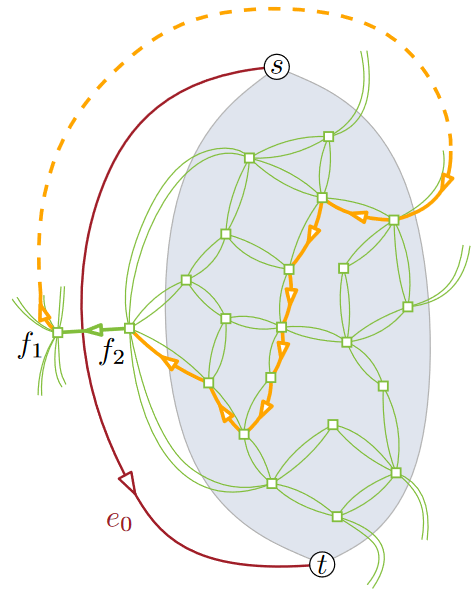
\includegraphics[width=0.3\textwidth]{images/max-flow-1.png}
	\end{center}
	\item Berechne daraus einen maximalen Fluss $\Phi$:
	$$\Phi(e)\coloneqq\text{dist}(f_1,\text{rechts}(e))-\text{dist}(f_1,\text{links}(e))$$
	\begin{center}
		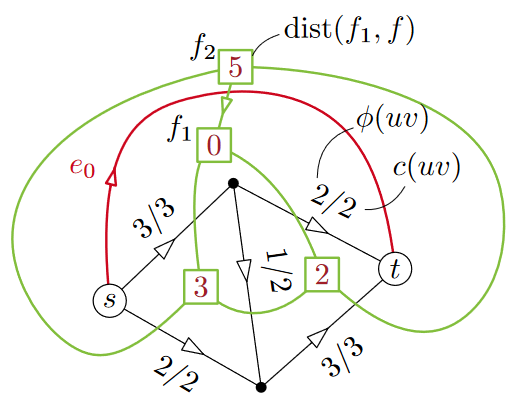
\includegraphics[width=0.3\textwidth]{images/max-flow-2.png}
	\end{center}
	\item Überprüfe Eigenschaften eines Flusses:
	\begin{itemize}
		\item Flusserhaltung: Für einen Knoten rechnet man im Kreis $\text{rechts}-\text{links}$, sodass sich rechts und links jeweils rauskürzen
		\item Zulässigkeit: Eine Möglichkeit von $f_1$ nach rechts$(uv)$ zu gehen, ist, zuerst von $f_1$ nach links$(uv)$ und dann über die Kante $e^*=(uv)^*$ nach rechts$(uv)$ zu gehen. Also ist 
		\begin{align*}
			&\vphantom{ } \text{dist}(f_1, \text{rechts}(uv))\leq \text{dist}(f_1, \text{links}(uv)) + c(uv) \\
			\iff{}& \text{dist}(f_1, \text{rechts}(uv)) - \text{dist}(f_1, \text{links}(uv)) \leq c(uv).
		\end{align*}
		\item Asymmetrie: Dies folgt aus links$(uv)=$ rechts$(vu)$ bzw. links$(vu)=$ rechts$(uv)$
	\end{itemize}
	\begin{center}
		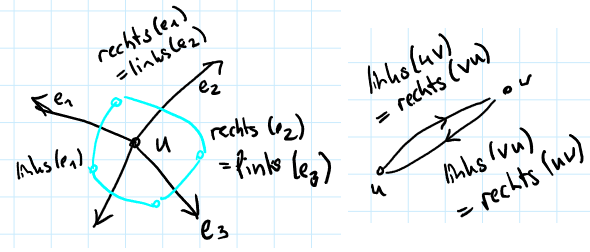
\includegraphics[width=0.4\textwidth]{images/max-flow-3.png}
	\end{center}
	\item Damit ist der Satz bewiesen.
\end{itemize}
\bigskip
Betrachte nun den allgemeinen Falls, dass $s$ und $t$ an beliebigen Facetten liegen:
\begin{itemize}
	\item Wähle einen gerichteten Pfad $P$ von $s$ nach $t$
	\item Sei $C^*\subseteq A^*$ ein gerichteter Kreis im Dualen und $C\subseteq A$ der entsprechende Schnitt im Primalen
	\item Ist $C^*$ ein $s$-$t$-Kreis, dann gilt $|C^*\cap P^*|=|C^*\cap {P^*}^{-1}|+1$, d.h. der Kreis geht einmal mehr von links nach rechts als von rechts nach links
	\item Ist $C^*$ ein $t$-$s$-Kreis, dann gilt $|C^*\cap P^*|=|C^*\cap {P^*}^{-1}|-1$
	\item Ansonsten gilt: $|C^*\cap P^*|=|C^*\cap {P^*}^{-1}|$
	\begin{center}
		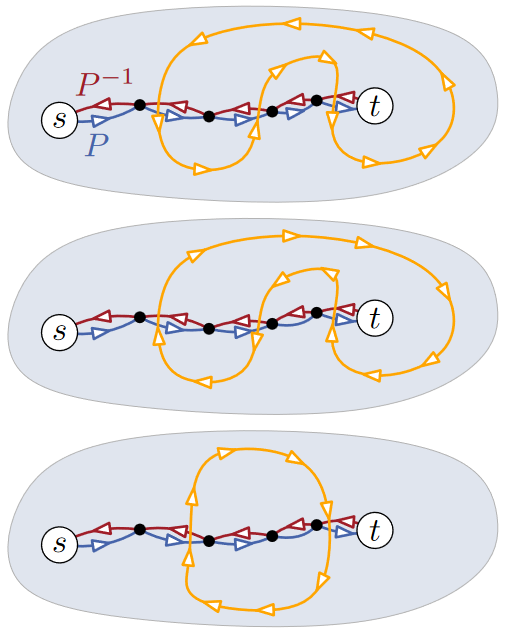
\includegraphics[width=0.3\textwidth]{images/max-flow-4.png}
	\end{center}
	\item Verringert man alle Kapazitäten der Kanten auf $P$ um $\alpha$ und erhöht alle Kapazitäten der Kanten auf $P^{-1}$ um $\alpha$, so wird
	\begin{itemize}
		\item jeder $s$-$t$-Kreis um genau $\alpha$ kürzer,
		\item jeder $t$-$s$-Kreis um genau $\alpha$ länger,
		\item jeder andere Kreis weder länger noch kürzer
	\end{itemize}
	\item Anfangs waren alle Kreislängen positiv. Wählt man $\alpha>0$ groß genug, werden Kreise negative Länge bekommen, aber nur $s$-$t$-Kreise!
	\item Ein Kreis, der bei kleinstem $\alpha$ negative Länge bekommt, ist ein kürzester $s$-$t$-Kreis
\end{itemize}

Finde jetzt also maximales $\alpha$ so, dass noch keine negative Kreise entstehen.

\textbf{Satz}: Dieses maximale $\alpha$ kann in $\mathcal{O}(n\log n)$ bestimmt werden. \qquad \textit{ohne Beweis}.

\textbf{Korollar}: \texttt{MAX-FLOW} in planaren Graphen kann in $\mathcal{O}(n\log n)$ berechnet werden.